%----------------------------------------------------------------------------------------
%	SECTION 1.1
%----------------------------------------------------------------------------------------

\section{Convexity and Jensen's Inequality.}

\begin{definition}
    A subset $K \subseteq E^n$, of a Euclidean space $E$ is said to be
    \textbf{convex} if for any two points in $K$, the line segment adjoining
    them is also in  $K$. That is for any  $x,y \in K$, the line
    $l(x,y)=tx+(1-t)y \in K$, for any $t \in [0,1]$.
\end{definition}

\begin{definition}
    Let $K \subseteq E^n$ be a subset of a Euclidean space $E$. We call a point
    $x \in K$ a \textbf{convex combination} of the points $x_1, \dots, x_n \in
    K$ if there exist scalars $a_1, \dots, a_n$ with $\sum{a_i}=1$ such that
    $\sum{a_ix_i}=x$. We call the set of all convex combinations of $K$ a
    \textbf{convex hull}.
\end{definition}

\begin{lemma}\label{1.2.1}
    A set $K$ is convex if, and only if every comvex combination of points of
    $K$ is also in  $K$.
\end{lemma}
\begin{proof}
    Suppose $K$ is convex. Then for any  $x,y \in K$, let $l(x,y)=xt+(1-t)y$ be
    the line adjoining $x$ and  $y$. Then  $l(x,y) \in K$ is a point of $K$
    which is a convex combination of  $x$ and  $y$.

    Now suppose that for any points  $x_1, \dots ,x_n \in K$, that their convex
    combination is also in $K$, suppose the same is true for the points $y_1,
    \dots y_n$; not necessarily the same convex combination as those for each
    $x_i$. Let $x=\sum{a_ix_i}$ and $y=\sum{b_iy_i}$ for scalars $a_i$,  $b_i$
    where  $1 \leq i \leq n$. Now consider the line  $l(x,y)=tx+(1-t)y$ for some
    $t \in [0,1]$. Then
    $l(x,y)=\sum{ta_ix_i}+\sum{(1-t)b_iy_i}=\sum{ta_ix_i+(1-t)b_iy_i}$. So
    $l(x,y)$ is a sum of convex combinations of the points $a_ix_i,b_iy_i \in K$
    for each  $i$; by hypothesis, this makes  $l(x,y) \in K$.
\end{proof}

\begin{figure}[h]
    \centering
    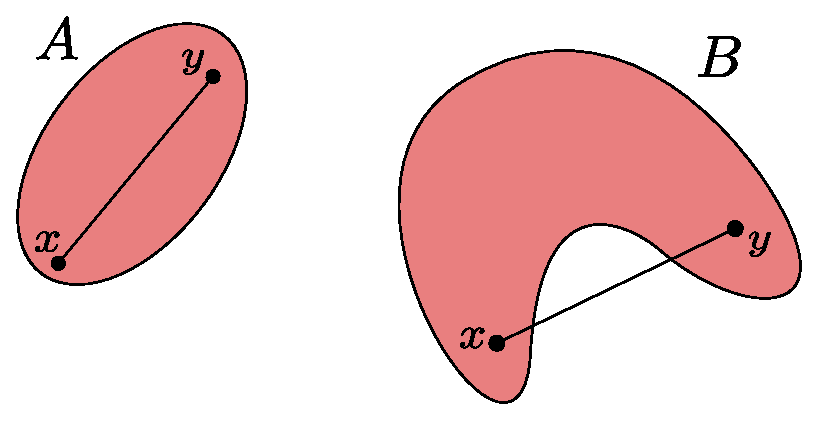
\includegraphics[scale=0.5]{Figures/Chapter1/convex.eps}
    \caption{A convex set, $A$ and a non-convex set  $B$.}
    \label{fig_1.1}
\end{figure}

\begin{figure}[h]
    \centering
    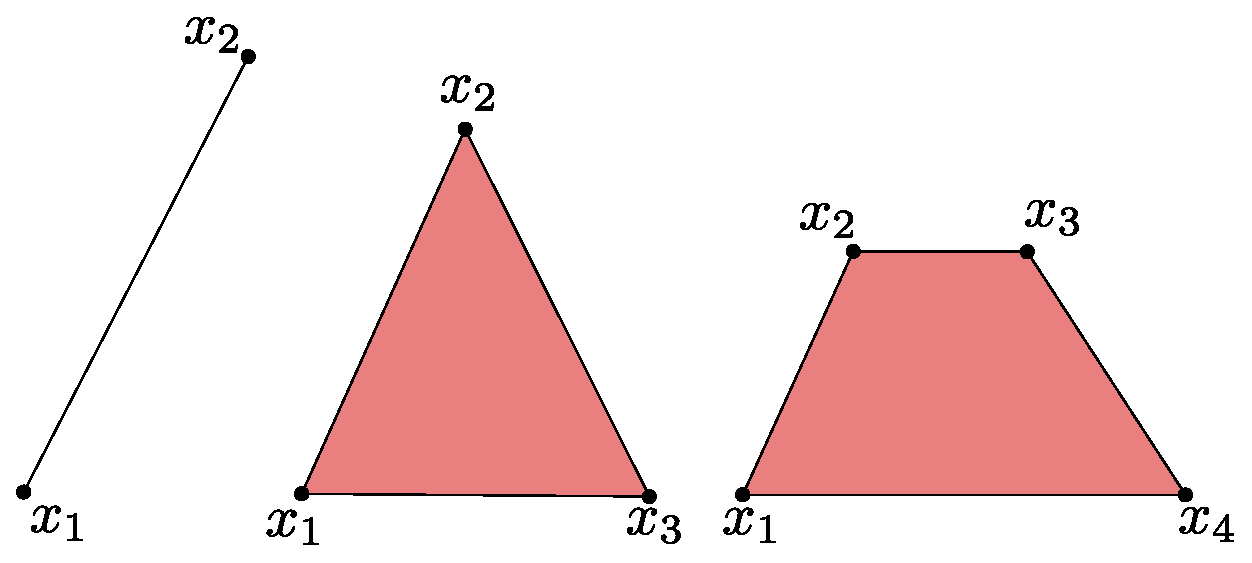
\includegraphics[scale=0.5]{Figures/Chapter1/convex_hulls.eps}
    \caption{$2$-dimensional convex hulls.}
    \label{fig_1.2}
\end{figure}

\begin{definition}
    Let $f$ be a real-valued function, and let  $K \subseteq \dom{f}$ be convex.
    We call $f$  \textbf{convex up} if, for every $x,y \in K$ and $t \in [0,1]$,
    \begin{equation}
        f(tx+(1-t)y) \leq tf(x)+(1-t)f(y)
    \end{equation}
    We call $f$  \textbf{convex down} if, for every $x,y \in K$ and $t \in
    [0,1]$,
    \begin{equation}
        f(tx+(1-t)y) \geq tf(x)+(1-t)f(y)
    \end{equation}
    If either equality is strict, i.e. $f(tx+(1-t)y) \neq tf(x)+(1-t)f(y)$ for
    some $x$ and  $y$, then we call  $f$  \textbf{strictly convex} (up or down).
\end{definition}

\begin{figure}[h]
    \centering
    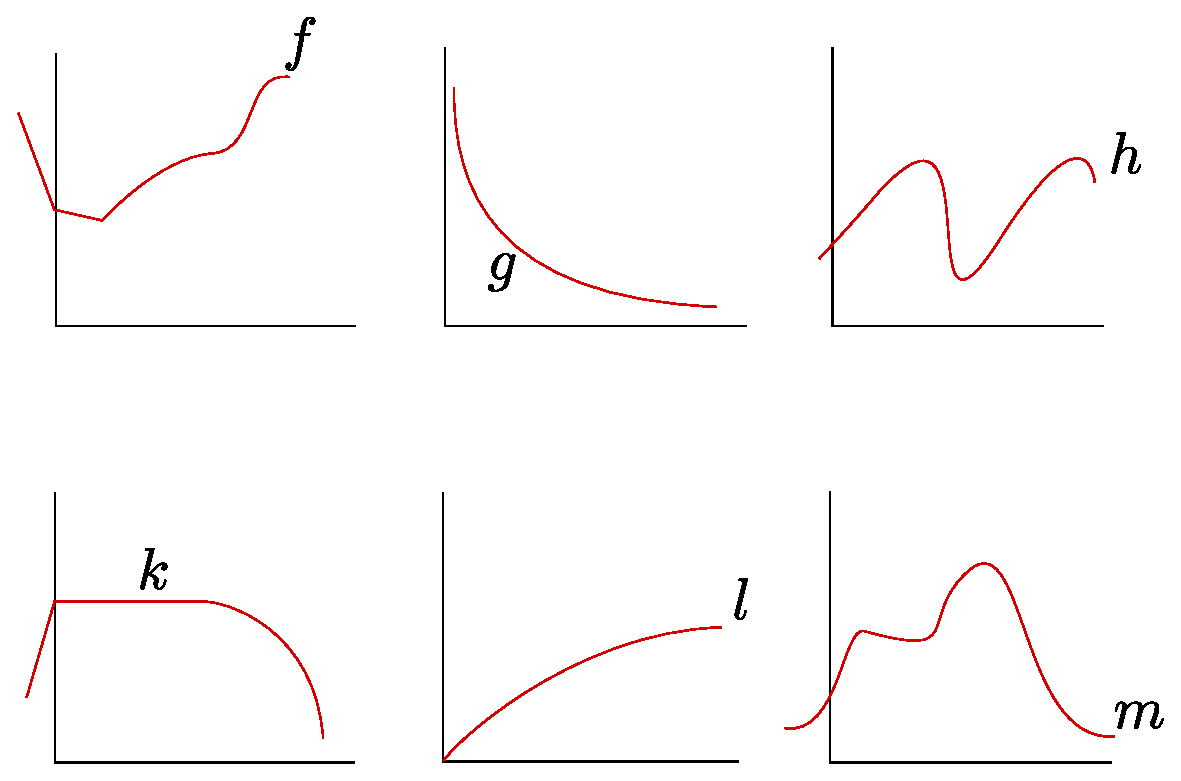
\includegraphics[scale=0.5]{Figures/Chapter1/convex_func.eps}
    \caption{The following are real-valued functions. The function $f$ is convex
        up, the function  $h$ is strictly convex up, while  $g$ is not convex.
        Similarly, $k$ is convex down, $l$ is strictly convex down, while  $m$ is
        not convex.
    }
    \label{fig_1.3}
\end{figure}

\begin{lemma}\label{1.2.2}
    If $f$ is a real-valued function, and  $K \subseteq \dom{f}$ is a convex
    open set, then if $f$ is convex (up or down), then $f$ is continuous.
\end{lemma}

\begin{example}
    The above lemma does not hold for closed sets. If $K=[0,1]$, and $f(x)=x$
    for all $x \in (0,1]$ and $f(0)=1$, then $f$ is discontinuous despite being
    convex up.
\end{example}

\begin{lemma}\label{1.2.3}
    If $f$ is a twice differentiable real-valued function with first derivative
    $f'(x)$ for every $x \in K$, then  $f$ is convex up if, and only if $f'$ is
    nondecreasing. Similarly,  $f$ is convex down if, and only if  $f'$ is
    nonincreasing.
\end{lemma}

\begin{theorem}[Jensen's Inequality]\label{1.2.4}
    Let $E$ be a Euclidean space, and let  $K$ be an interval in  $E^1$. Let
    $F(x)$ be a probaility distribution concentrated on $K$, and  $X$ be the
    associated random variable with the prpbality  $P(X \leq x)=F(x)$. Then if
    the expectation $E(X)$ exists, and if $f$ is a function that is convex up,
    then:
    \begin{equation}
        E(f(X)) \geq f(E(X))
    \end{equation}
    If $f$ is convex down, then:
    \begin{equation}
        E(f(X)) \leq f(E(X))
    \end{equation}
    If $f$ is strictly convex, then $(1.14)$ and $(1.15)$ are strict, except
    possibly when $P(X=x_0)=1$ for some $x_0 \in K$.
\end{theorem}

\begin{figure}
    \centering
    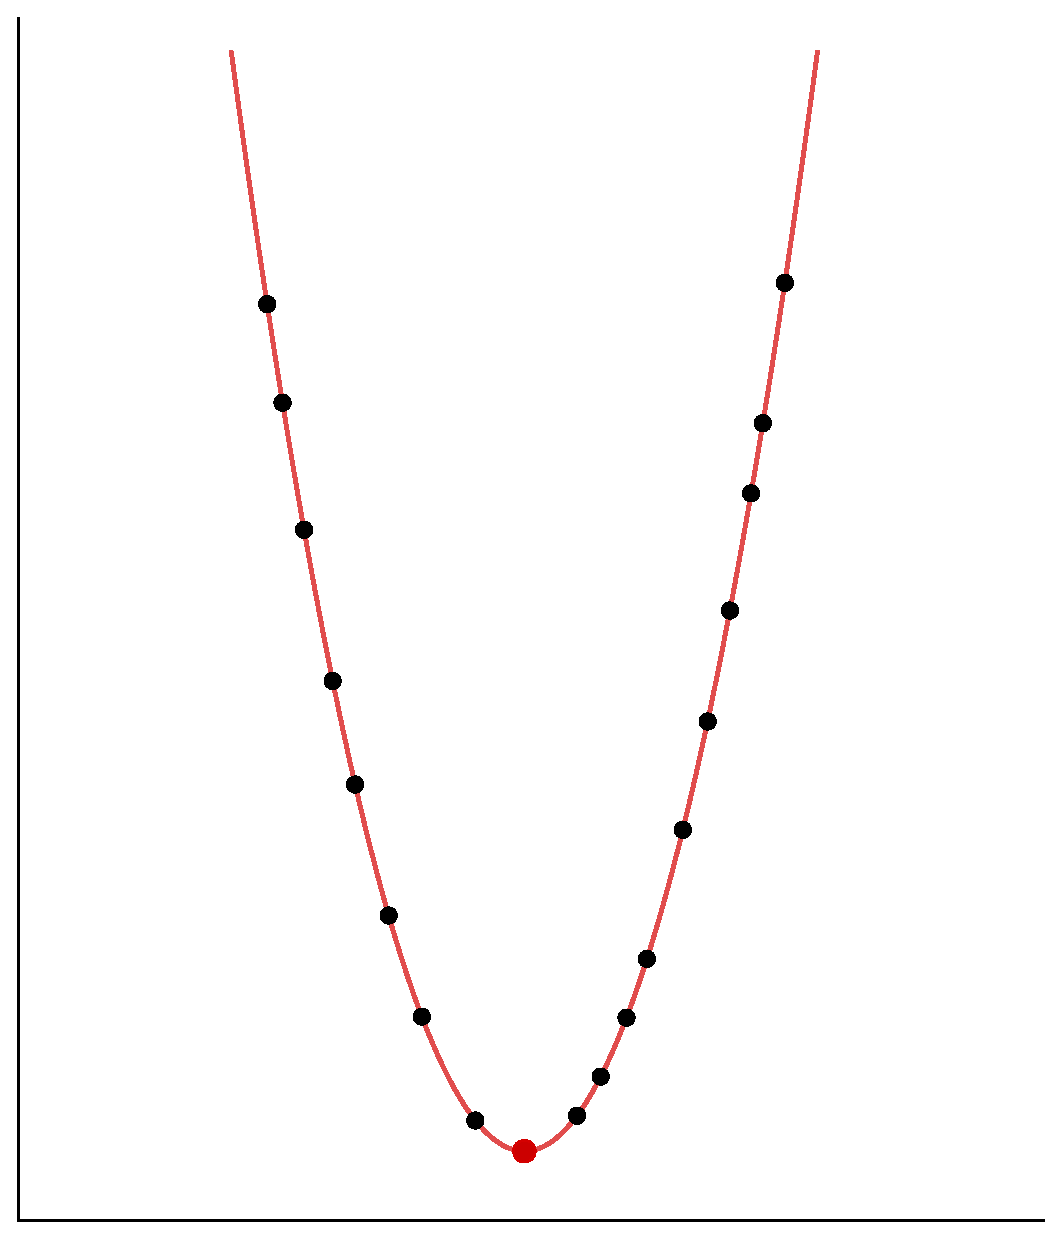
\includegraphics[scale=0.2]{Figures/Chapter1/jensen_ineq.eps}
    \caption{Jensen's Inequality says that if a mass distribution is placed on
    the graph of the given function, then the center of mass lies above, or on
    the graph.
    }
    \label{fig_1.4}
\end{figure}

We now finish the section by introdicing examples of Jensen's inequality
with probability distributions. There are two accompying theorems, and one is
the continuous analog of the other.

\begin{example}
    Let $S=\{s_1, s_2, \dots\} \subseteq \R$ be a discrete sample
    space of real numbers. Let $p(s_i)$ be a nonnegative function such
    that $\sum{p(s_i)}=1$. Let $1(s_i)$ be any other nonnegative function
    defined on $S$, and define the random variable $X$ by:
    \begin{equation*}
        X(s)=\frac{q(s)}{p(s)}
    \end{equation*}
    for any $s \in S$. THen by Jensen's inequality we have $E(\log(X))
    \leq \log{E(X)}$, which gives the following inequality:
    \begin{equation*}
        \sum{p(s_i)\log{\frac{1}{p(s_i)}}} \leq
        \sum{p(s)\log{\frac{1}{q(s)}}}+\log{\alpha}
    \end{equation*}
    where $\alpha=\sum{q(s_i)}$.

    Furthermore, $\log{x}$ is strictly convex down, so equality holds
    if, and only if $X=\beta$ for some constant  $\beta$. Since
    $\sum{p(s_i)}=1$, we get $\beta=\alpha$, and so equality holds if,
    and only if  $q(s_i)=\alphap(s_i)$ for all $i$ such that  $p(s_i)
    \neq 0$.
\end{example}

\begin{theorem}\label{1.2.5}
    Let $\{p_i\}_{i \in \Z}$ be a sequence of positive real numbers such that
    $\sum{p_i}=1$. If $\{q_i\}$ is any other sequence of nonegative reals with
    $\sum{q_i}=\alpha$, then:
    \begin{equation}
        \sum{p_i\log{\inv{p_i}}} \leq\sum{p_i\log{\inv{q_i}}}+\log{\alpha}
    \end{equation}
    with equality hilding if, and only if $q_i=\alpha p_i$ for all  $i$.
\end{theorem}

\begin{example}
    Take $S=\R$, and let  $p(x)$ be a nonnegative density function such that
    $\int_{-\infty}^{\infty}{p(x)} \ \dd{x}=1$. Then $p$ induces a probability
    measure on  $S$. Now, let  $q(x)$ be any other nonnegative function defined
    on $S$ and define the random variable  $X$ as was in example $1.3$. Then,
    again by Jensen's inequalty, we get:
    \begin{equation*}
        \int_{-\infty}^{\infty}{p(x)\log{\frac{q(x)}{p(x)}}} \ \dd{x} \leq
        $\log{\int_{I}{q(x)}} \ \dd{x}$
    \end{equation*}
    where $I$ is a measurable subset of $\R$.
\end{example}

\begin{theorem}\label{1.2.6}
    Let $I$ be a measurable subset of  $\R$ and let  $p(x)$ be a positive
    function defined on $I$, with  $\int_{I}{p(x)} \ \dd{x}=1$. If $q(x)$ is a
    nonnegative positive function defined on $I$ with  $\int{q(x)} \
    \dd{x}=\alpha$, then:
    \begin{equation}
        \int_{I}{p(x)\log{\inv{p(x)}}} \ \dd{x} \leq
        \int_{I}{p(x)\log{\inv{q(x)}}}+\log{\alpha}
    \end{equation}
    with equality holding if, and only if $q(x)=\alpha p(x)$.
\end{theorem}
